\chapter{Extended Campaign and Universe}

\section{Old Gods}

The old gods exist prior to the Celestials and well known gods of the world. These gods have an origin that could be from any point in history and from any place in history far before the existence of modern life on Orilla. These gods were of the first ascended beings in the universe. the Old gods of Orilla have lived for what could be seen as eternity and have long since decided to slumber and not interact with the mortal realm. Their power and abilities are far superior to any other beings in the universe and even as they slumber they can still greatly influence the mortal realms and even that of the ascended beings (modern gods).

\subsection{Yogg'Saron}

Yogg'Saron\footnote{Modeled after Yogg'Saron from World of Warcraft.} is an old god based on insanity. Yogg'Saron has been slumbering for the entire entire existence of life on Orilla. Even though he has been slumbering, his influence is so great that some creatures in the past have been driven insane by his mental influence and became servants embodying his essence in physical form. These servants have caused destruction and chaos throughout ancient times and left remnants of power that can still be found today. 

Yogg'Saron's most powerful influence was through a great beast that is believed by many to have been the entire essence of Yogg. The beast was vanquished by an army of highly trained soldiers with the help of a demigod Ursoc, whom described him as ``the beast with a thousand maws.'' The beast had such a strong influence from Yogg, that the blood of the creature was used for forging great and powerful items following the beasts defeat. Unfortunately, as the blood was also influenced by Yogg, the items created with the beasts blood have an inherent connection to Yogg.

\begin{center}
	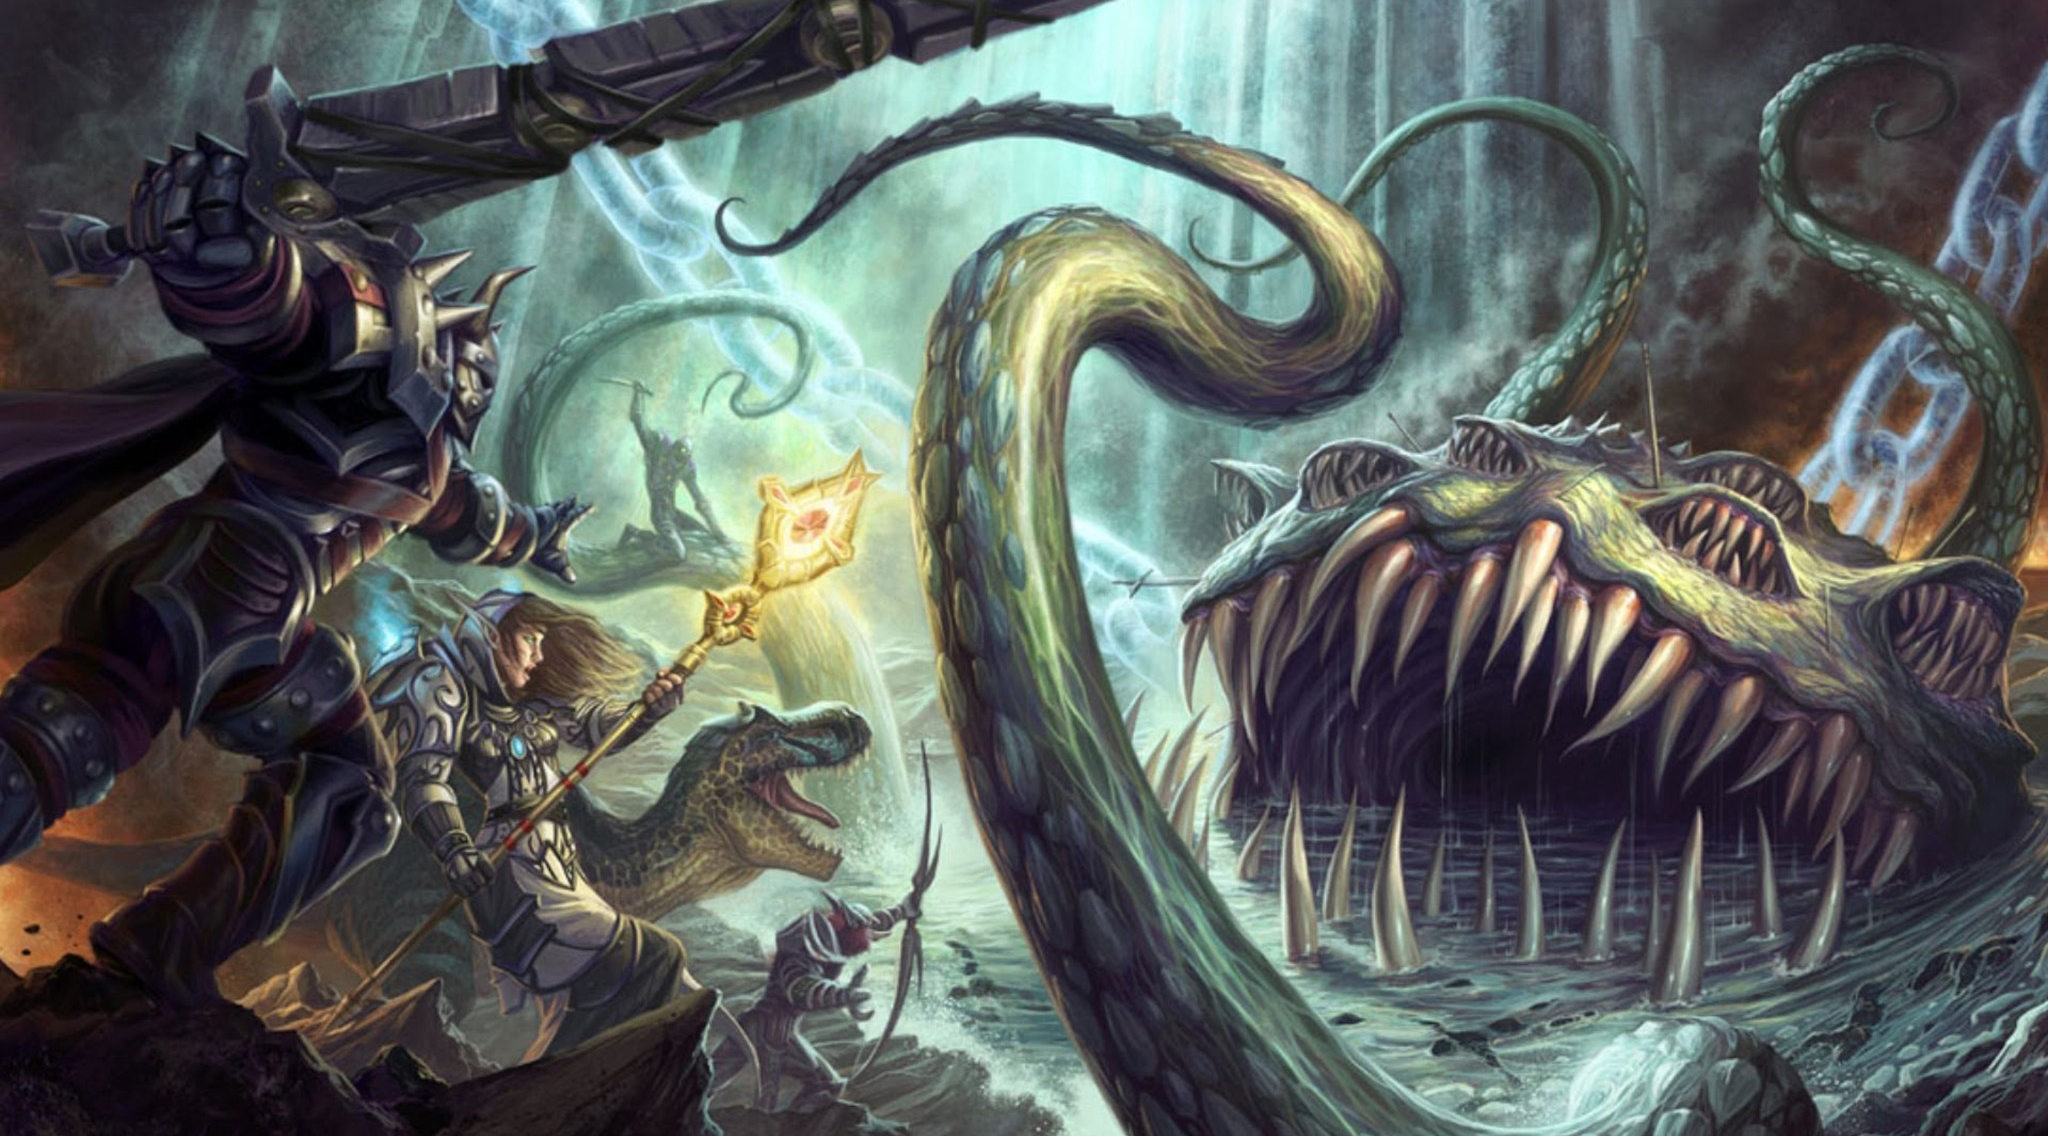
\includegraphics[width=\linewidth]{img/WoW/yogg-saron.jpg}
\end{center}

Yogg'Sarons existence is believed to be unknown to most of the inhabitants of Orilla. However, Yogg's power is so vast that the maddening, destructive taint seeps from its resting place and appears to tear at the sanity of an unknown number of Orilla's inhabitants. Because of this, Yogg possess worshipers across all the world's peoples and cultures.

\subsubsection{Yogg'Saron Puzzle Box}

The Yogg'Saron puzzle box\footnote{From https://wowwiki.fandom.com/wiki/Puzzle\_Box\_of\_Yogg-Saron} is an artifact that was created with a connection to Yogg'Saron. The box is magically sealed and contains many shifting panels, hidden hinges, changing sides, magical barriers and more. The box is made of an allow of hardened Yogg'Saron blood and a substance called Katchin\footnote{Katchin from Dragonball Z.}, which is one of the hardest materials in the universe. The box is indestructible and appears impossible to actually solve and open. When attempting to open the box, the box will whisper messages to you to try and drive the user to insanity. 

\begin{multicols}{2}
	\begin{itemize}
		\item At the bottom of the ocean even light must die
		\item The silent, sleeping, staring houses in the backwoods always dream. It would be merciful to tear them down.
		\item There is no sharp distinction between the real and the unreal.
		\item Even death may die.
		\item There is a little lamb lost in dark woods.
		\item All places, all things have souls. All souls can be devoured.
		\item What can change the nature of a man?
		\item The stars sweep chill currents that make men shiver in the dark.
		\item You will all be alone in the end.
		\item Do you dream while you sleep or is it an escape from the horrors of reality?
		\item Look around. They will all betray you. Flee screaming into the black forest.
		\item In the land of Ny'alotha there is only sleep.
		\item In the sleeping city of Ny'alotha walk only mad things.
		\item Ny'alotha is a city of old, terrible, unnumbered crimes.
		\item Y'knath k'th'rygg k'yi mrr'ungha gr'mula.
		\item The void sucks at your soul. It is content to feast slowly.
		\item The drowned god's heart is black ice.
		\item It is standing right behind you. Do not move. Do not breathe.
		\item Have you had the dream again? A black goat with seven eyes that watches from the outside.
		\item In the sunken city, he lays dreaming.
		\item Open me! Open me! Open me! Then only will you know peace.
		\item You resist. You cling to your life as if it actually matters. You will learn.
		\item The tortured spirits of your ancestors cling to you, screaming in silence. Apparently they are quite numerous.
		\item The fish know all the secrets. They know the cold. They know the dark.
		\item The giant rook watches from the dead trees. Nothing breathes beneath his shadow.
		\item Beneath the shadow of the darkened spire, there is no light, no mercy, only void, and the chaos within. 
		\item They are coming for you...
		\item Give in to your fear...
		\item Kill them all... before they kill you...
		\item They have turned against you... now, take your revenge...
		\item It WAS your fault...
		\item Tell yourself again that these are not truly your friends...
		\item You are a pawn of forces unseen...
		\item There is no escape... not in this life... not in the next... 
		\item Trust is your weakness...
		\item Hope is an illusion...
		\item All that you know will fade...
		\item You will be alone in the end... 
	\end{itemize}
\end{multicols}

